\subsection{\textit{Rotordynamic Open-Source Software} - ROSS}
\label{sec:ross}

O \textit{Rotordynamic Open-Source Software}\footnote{\href{ross.readthedocs.io}{Link de acesso: ross.readthedocs.io}} (\textit{ROSS}) é uma biblioteca, feita em \textit{Python}, para modelagem e análises de dinâmica de rotação. Este é um código aberto específico, proposto por \citeonline{timbo2020} em parceria da Petrobras, UFRJ e UFU. A modelagem feita no \textit{ROSS} é baseada no que é apresentado por \citeonline{timbo2018} e utiliza como referência \citeonline{Friswell2010}. 

A modelagem e as análises são realizadas utilizando o Método dos Elementos Finitos (MEF). No caso, o \textit{ROSS} utiliza 6 graus de liberdade (\textit{gdl}) por nó, sendo 3 translações e 3 rotações, de acordo com a Equação \ref{Eq:dof}. A resolução das equações de movimento pode ser feita a partir do Método de \citeonline{newmark} ou pela metodologia de solução linear (\textit{LSIM}) do módulo \textit{Scipy} do \textit{Python}.

A diferença entre a modelagem proposta por \citeonline{Friswell2010} e \citeonline{Lalanne1998} está na orientação e posicionamento do eixos cartesianos. A Figura \ref{subfigure:coord} apresenta a diferença de eixos coordenados entre esses dois autores. 
\begin{figure}[H]
	\centering
	\caption{Subfiguras}
	\label{subfigure:coord}
	
	\begin{minipage}{0.8\textwidth}
		\centering
		
		\begin{subfigure}{0.4\textwidth}
			\centering
			\caption{Eixos Coordenados de \citeonline{Lalanne1998}}
			\label{fig:rot_lalanne}
			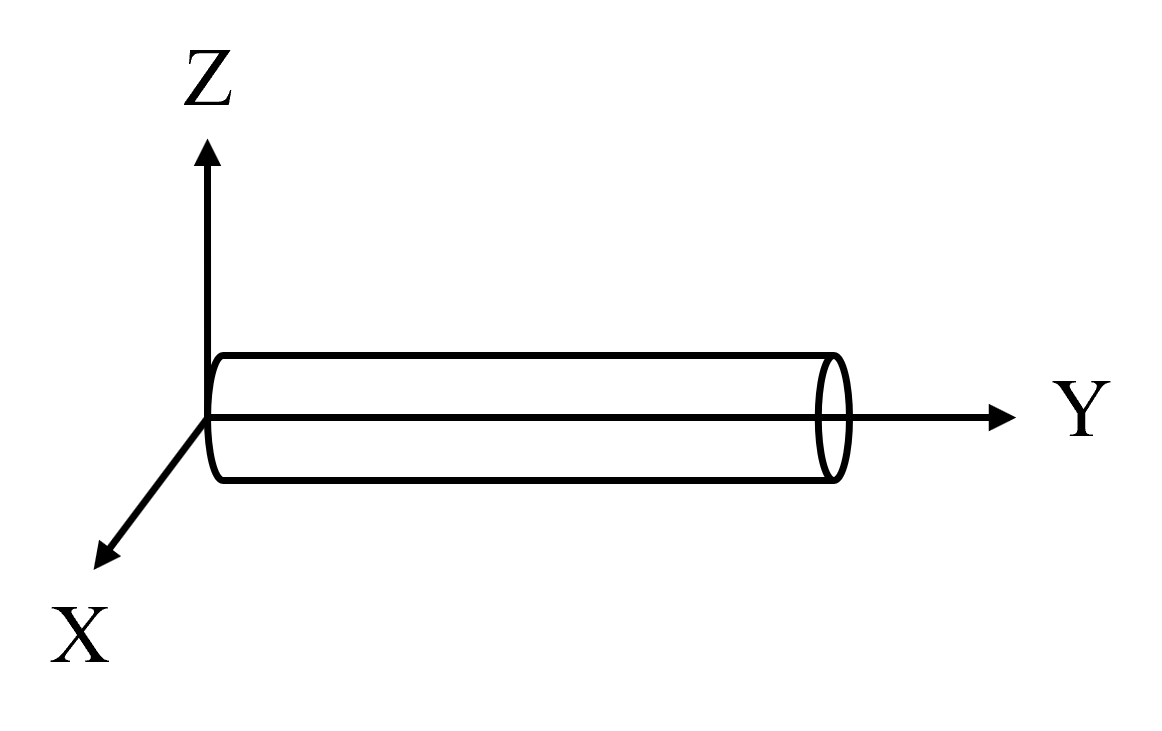
\includegraphics[width=\linewidth]{figuras/rot_lalanne.png}
		\end{subfigure}
		\hspace{10pt}
		\begin{subfigure}{0.33\textwidth}
			\centering
			\caption{Eixos Coordenados de \citeonline{Friswell2010}}
			\label{fig:rot_fris}
			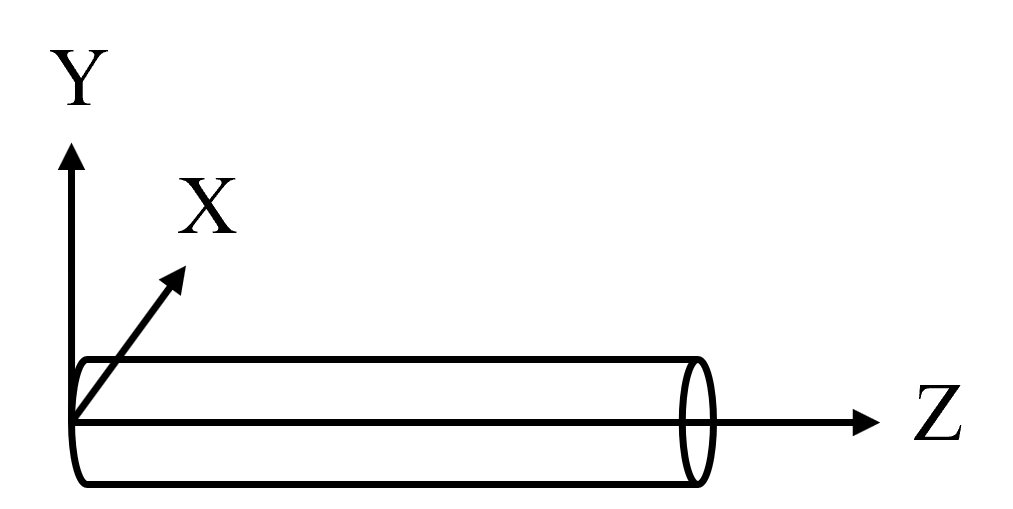
\includegraphics[width=\linewidth]{figuras/rot_fris.png}
		\end{subfigure}
		
		\par\vspace{0.5em}
		\raggedright
		{\small Fonte: Elaborado pelo autor.}
	\end{minipage}
\end{figure}

\citeonline{jessica2025} mostra que a modelagem de um sistema rotativo dividida entre os modelos de eixos, mancais e selos, discos e engrenagens e elementos de acoplamento. A seguir é apresentado sobre cada um desses elementos e sua modelagem.
\begin{itemize}
	\item \texttt{ShaftElement}: Responsável pelo cálculo das matrizes de rigidez $[K]$, massa $[M]$ e efeito giroscópico $[G]$ distribuídas do eixo considerando o material e os diâmetros internos e externos dos lados esquerdos e direitos do elemento de eixo.. O pacote utiliza a Teoria de Vigas de \citeonline{timoshenko1922}, o que considera não apenas a flexão pura (como na teoria de Euler-Bernoulli), mas também as deformações por cisalhamento e a inércia rotacional de seções transversais curtas. 
	\item \texttt{BearingElement} e \texttt{SealElement}: Implementa o suporte dos mancais e os selos nos nós pertinentes. Esta classe permite associar coeficientes de rigidez ($k_{xx}, k_{yy}$) e amortecimento ($c_{xx}, c_{yy}$) estáticos ou variantes com a velocidade de rotação $\Omega$. Além disso, podem ser considerado os coeficientes cruzados, que relacionam as direções $xy$, $xz$ e $yz$. Portanto, este elemento contribui somente com as matrizes de rigidez $[K]$ e amortecimento $[C]$.
	\item \texttt{DiskElement}: Modela elementos concentrados em nós específicos, adicionando propriedades de massa ($m$), momento de inércia polar ($I_p$) e momento de inércia diametral ($I_d$) influenciando nas matrizes de massa $[M]$ e efeito giroscópico $[G]$. 
	\item \texttt{GearElement} e \texttt{GearElementTVMS}: São classes filhas da \texttt{DiskElement} e, portanto, contribuem para o sistema da mesma maneira. Entretanto, para a sua definição são exigidos parâmetros geométricos e de engrenamento específicos para engrenagens. Entre essas variáveis, coloca-se, módulo, ângulo de pressão, ângulo de hélice, número de dentes, diâmetro primitivo entre outras. 
\end{itemize}

Dessa forma, com os modelos de cada componente é possível juntá-los e fazer a modelo do sistema rotativo completo. No caso de sistemas engrenados são necessários dois ou mais rotores com engrenagens e então deve-se juntá-los com a função do \texttt{MultiRotor} \cite{jessica2025}.
A Figura \ref{fig:multirotor_ex} apresenta um exemplo de modelagem de um conjunto de rotores no \textit{ROSS}.
\begin{figure}[H]
	\centering
	\caption{Exemplo de rotores engrenados no \textit{ROSS}}
	\label{fig:multirotor_ex}
	
	\begin{minipage}{0.8\textwidth}
		\centering
		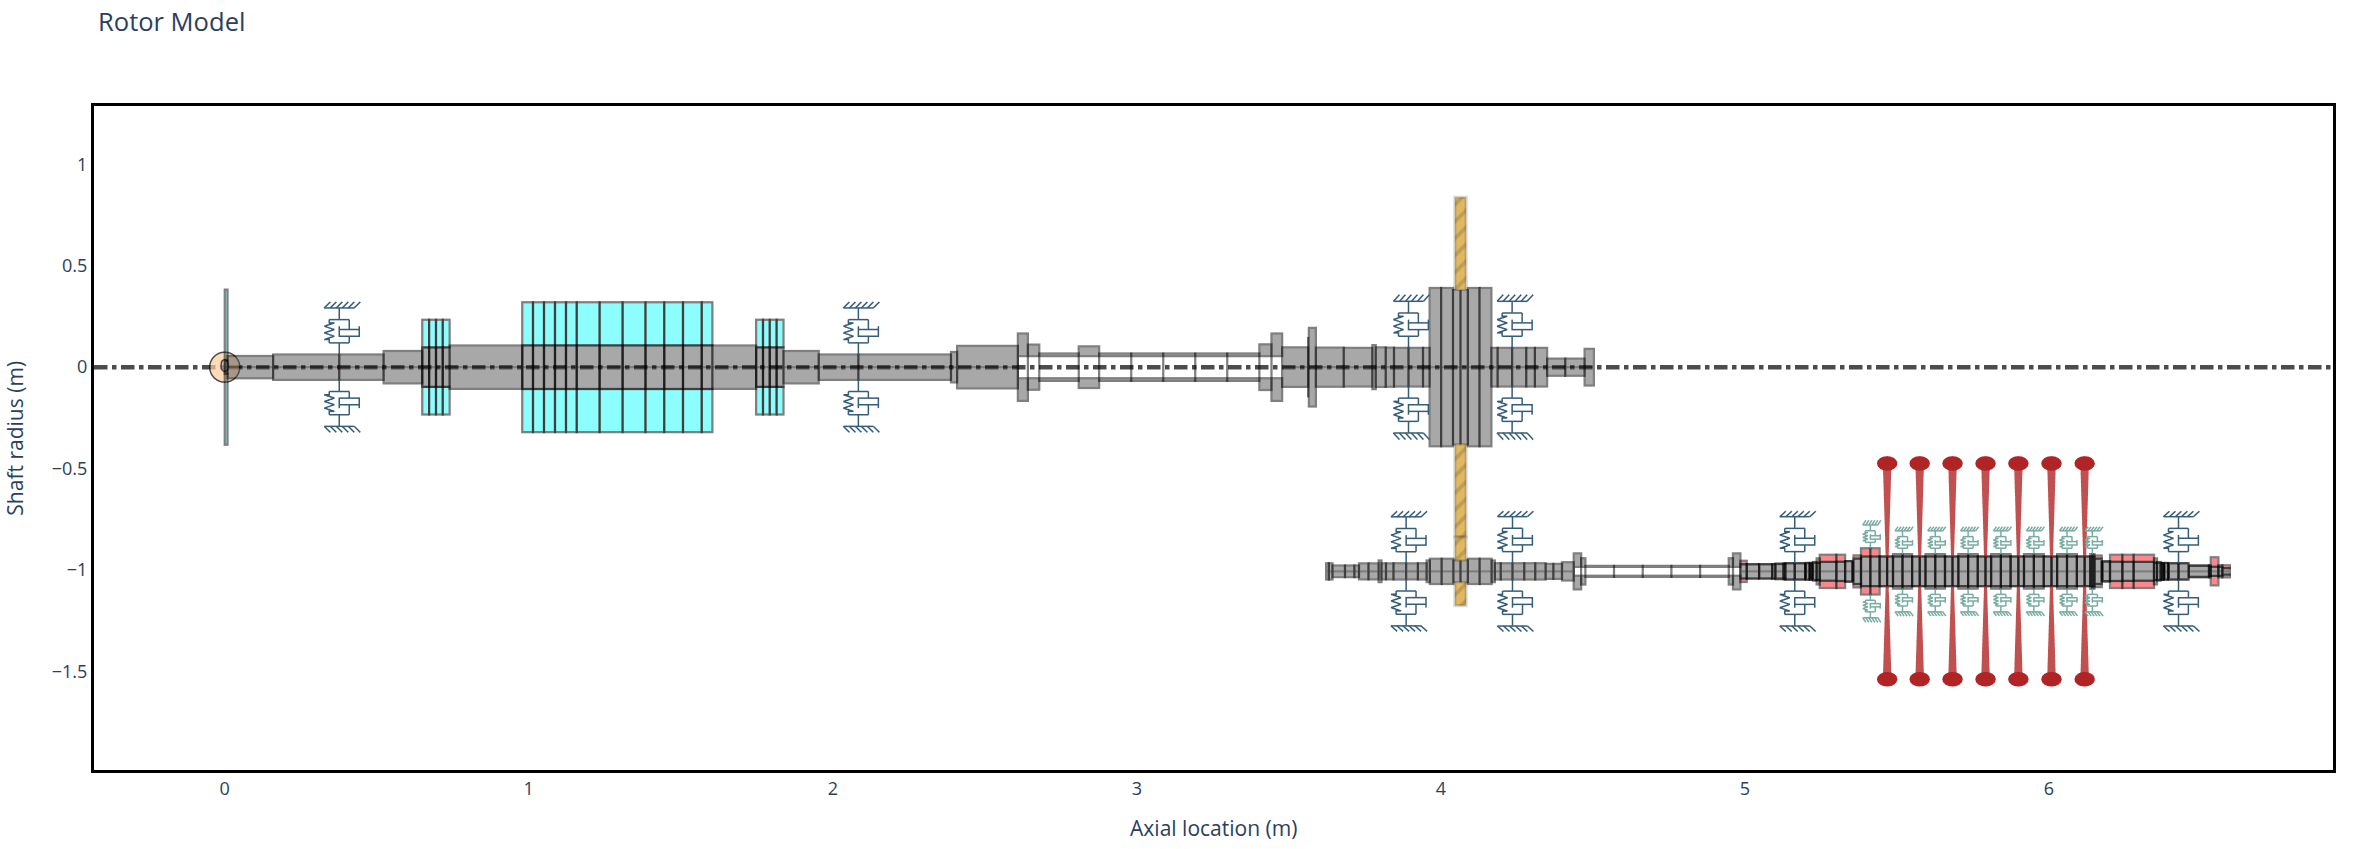
\includegraphics[width=\linewidth]{figuras/multirrotor_completo.png}
		\par\vspace{0.3em}
		\raggedright
		{\small Fonte: Elaborado pelo autor.}
	\end{minipage}
\end{figure}

Na Figura \ref{fig:multirotor_ex} observa-se diferentes elementos de eixo na cor cinza, ainda com variação do material representado pela cor ciano. Nota-se ainda os elementos de mancais e selos com a simbologia de rigidez e amortecimento e além disso, os discos em vermelho e engrenagem em amarelo. 

Com a modelagem feita, é possível realizar diversas análises do sistema rotativo simples ou com multi rotores, entre elas a obtenção de resposta de vibração no tempo, órbitas, desbalanceamento, função de reposta em frequência (FRF), mapa de velocidade crítica sem amortecimento (UCS), Diagrama de Campbell, análise estática, análise modal, entre outras. Além disso, é possível executar casos de falhas como desalinhamento, trinca e roçamento.
A Figura \ref{fig:ross_analises} apresenta exemplo de de análises que podem ser feitas no \textit{ROSS}, como o UCS, análise de desbalanceamento e modos de vibrar.
\begin{figure}[H]
	\centering
	\caption{Exemplo de Análises no \textit{ROSS}}
	\label{fig:ross_analises}
	
	\begin{minipage}{0.8\textwidth}
		\centering
		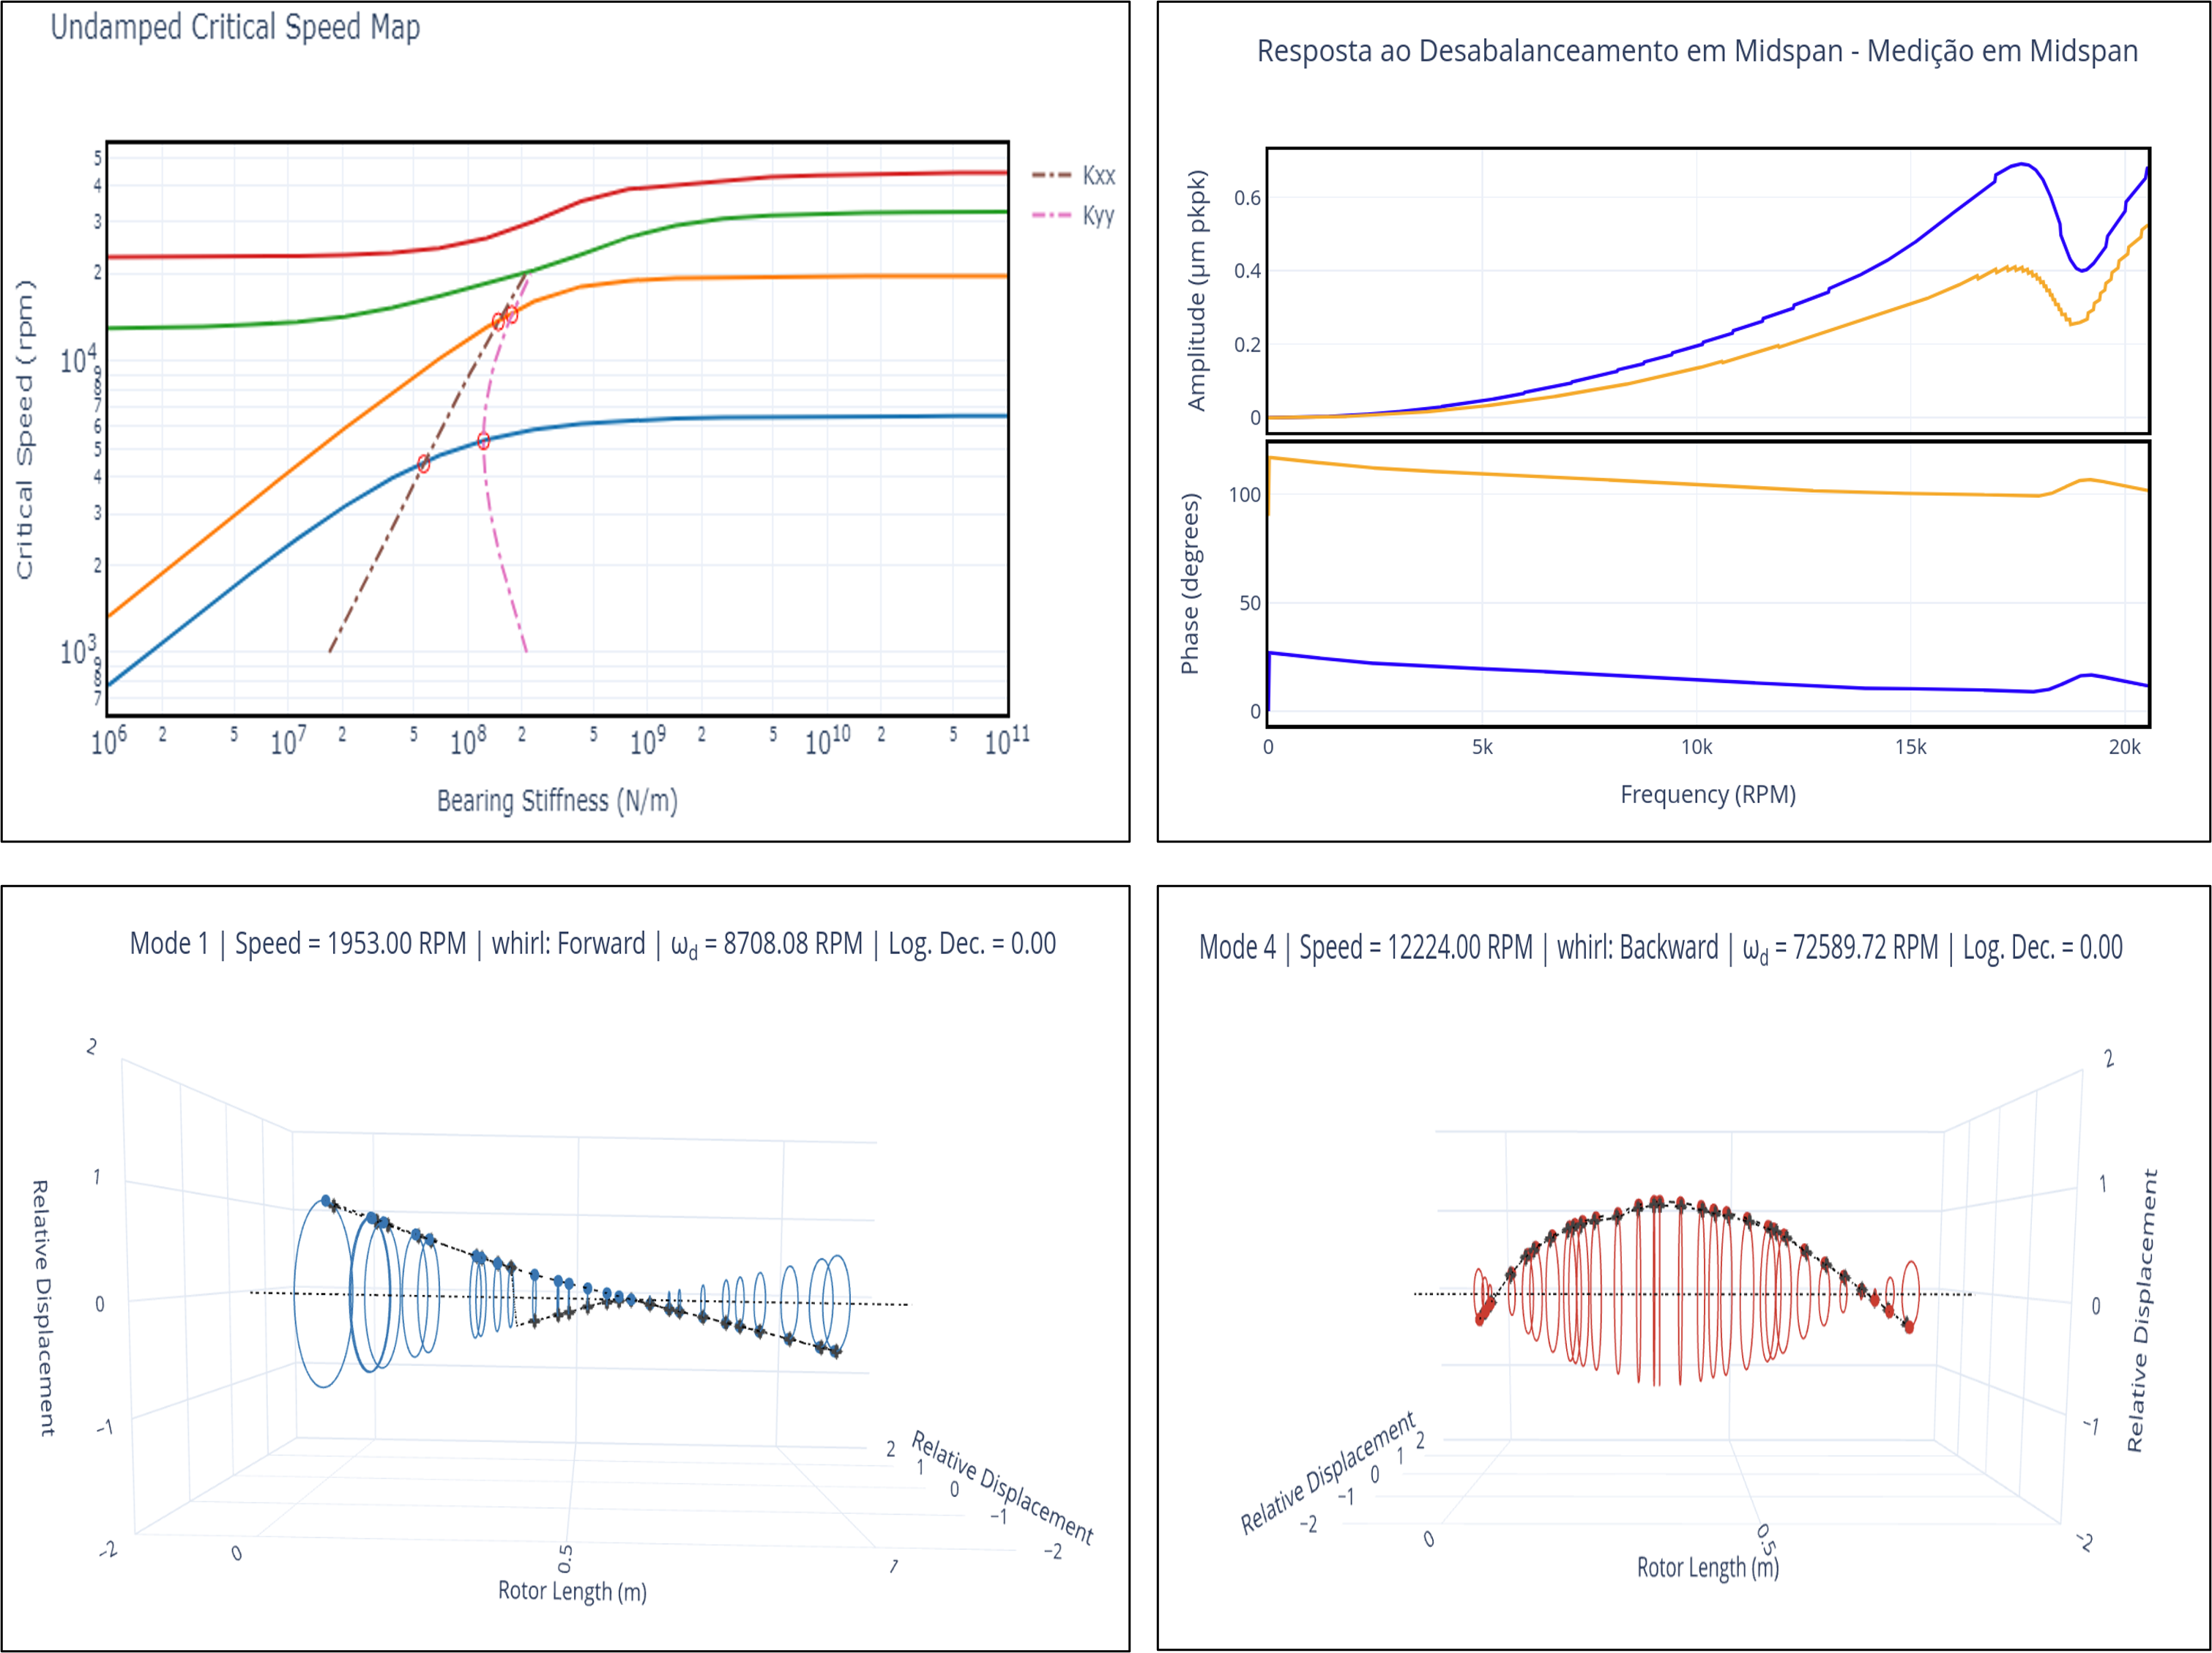
\includegraphics[width=\linewidth]{figuras/ross_analise.png}
		\par\vspace{0.3em}
		\raggedright
		{\small Fonte: Elaborado pelo autor.}
	\end{minipage}
\end{figure}

